% !TEX root = ../thesis.tex
\chapter{Discussion}
\label{chapter:discussion}

\section{Summary}
The ultimate objective of this thesis is to endow robots with nonverbal communication skills, to make them genuinely interact with humans. This thesis argues that a solution to achieve the goal is by exploiting computational methods and machine learning techniques, leveraging a large-data data containing the social signals that humans use in actual social communications. This thesis directly tackles the fundamental hurdle, the lack of available such dataset, by building the Panoptic Studio, one of the most complicated sensor systems to sense human motions (Chapter~\ref{chapter:system}). Leveraging the sensor system, this thesis presents the state-of-the-art measurement method to capture a broad spectrum of social signals of interacting individuals, including the motions from faces, bodies, and hands (Chapters~\ref{chapter:trajectory}, \ref{chapter:mocap}, and  \ref{chapter:totalcapture}). Our system and reconstruction method enable us to build a large-scale 3D motion capture corpus capturing various behavioral cues of interacting people, for the first time in the history (Chapter~~\ref{chapter:dataset}). The final part of this thesis computationally verifies that social signals are highly correlated and predictive each other, and introduces a social signal prediction task as a way to modeling nonverbal communication in a data-driven manner (Chapter~~\ref{chapter:prediction}).

This thesis demonstrates that the face, body, and hands motion of freely interacting groups can be markerlessly captured with a sufficient amount of sensors by applying ML-based measurement techniques for each view and consolidating them together. This is a crucial step showing the potential that the markerless motion capture approaches can outperform the popular marker-based motion capture method in the near future, which struggles in handling occlusions causing broken trajectories. 

As another important contribution, this thesis also demonstrates that the data captured in the lab environment can be used as a valuable source for the computer vision and machine learning algorithms applied in-the-wild. For example, our system enables to build the first widely used 2D hand keypoint detector~\cite{simon2017hand}. Our system also enables us to build the first 3D deformable human model with the expressive power for face, body, and hands.  Our dataset containing paired 3D motion annotation for each RGB image also allows us to build the first monocular total capture system~\cite{Xiang2019}. 


\begin{figure*}[t]	
	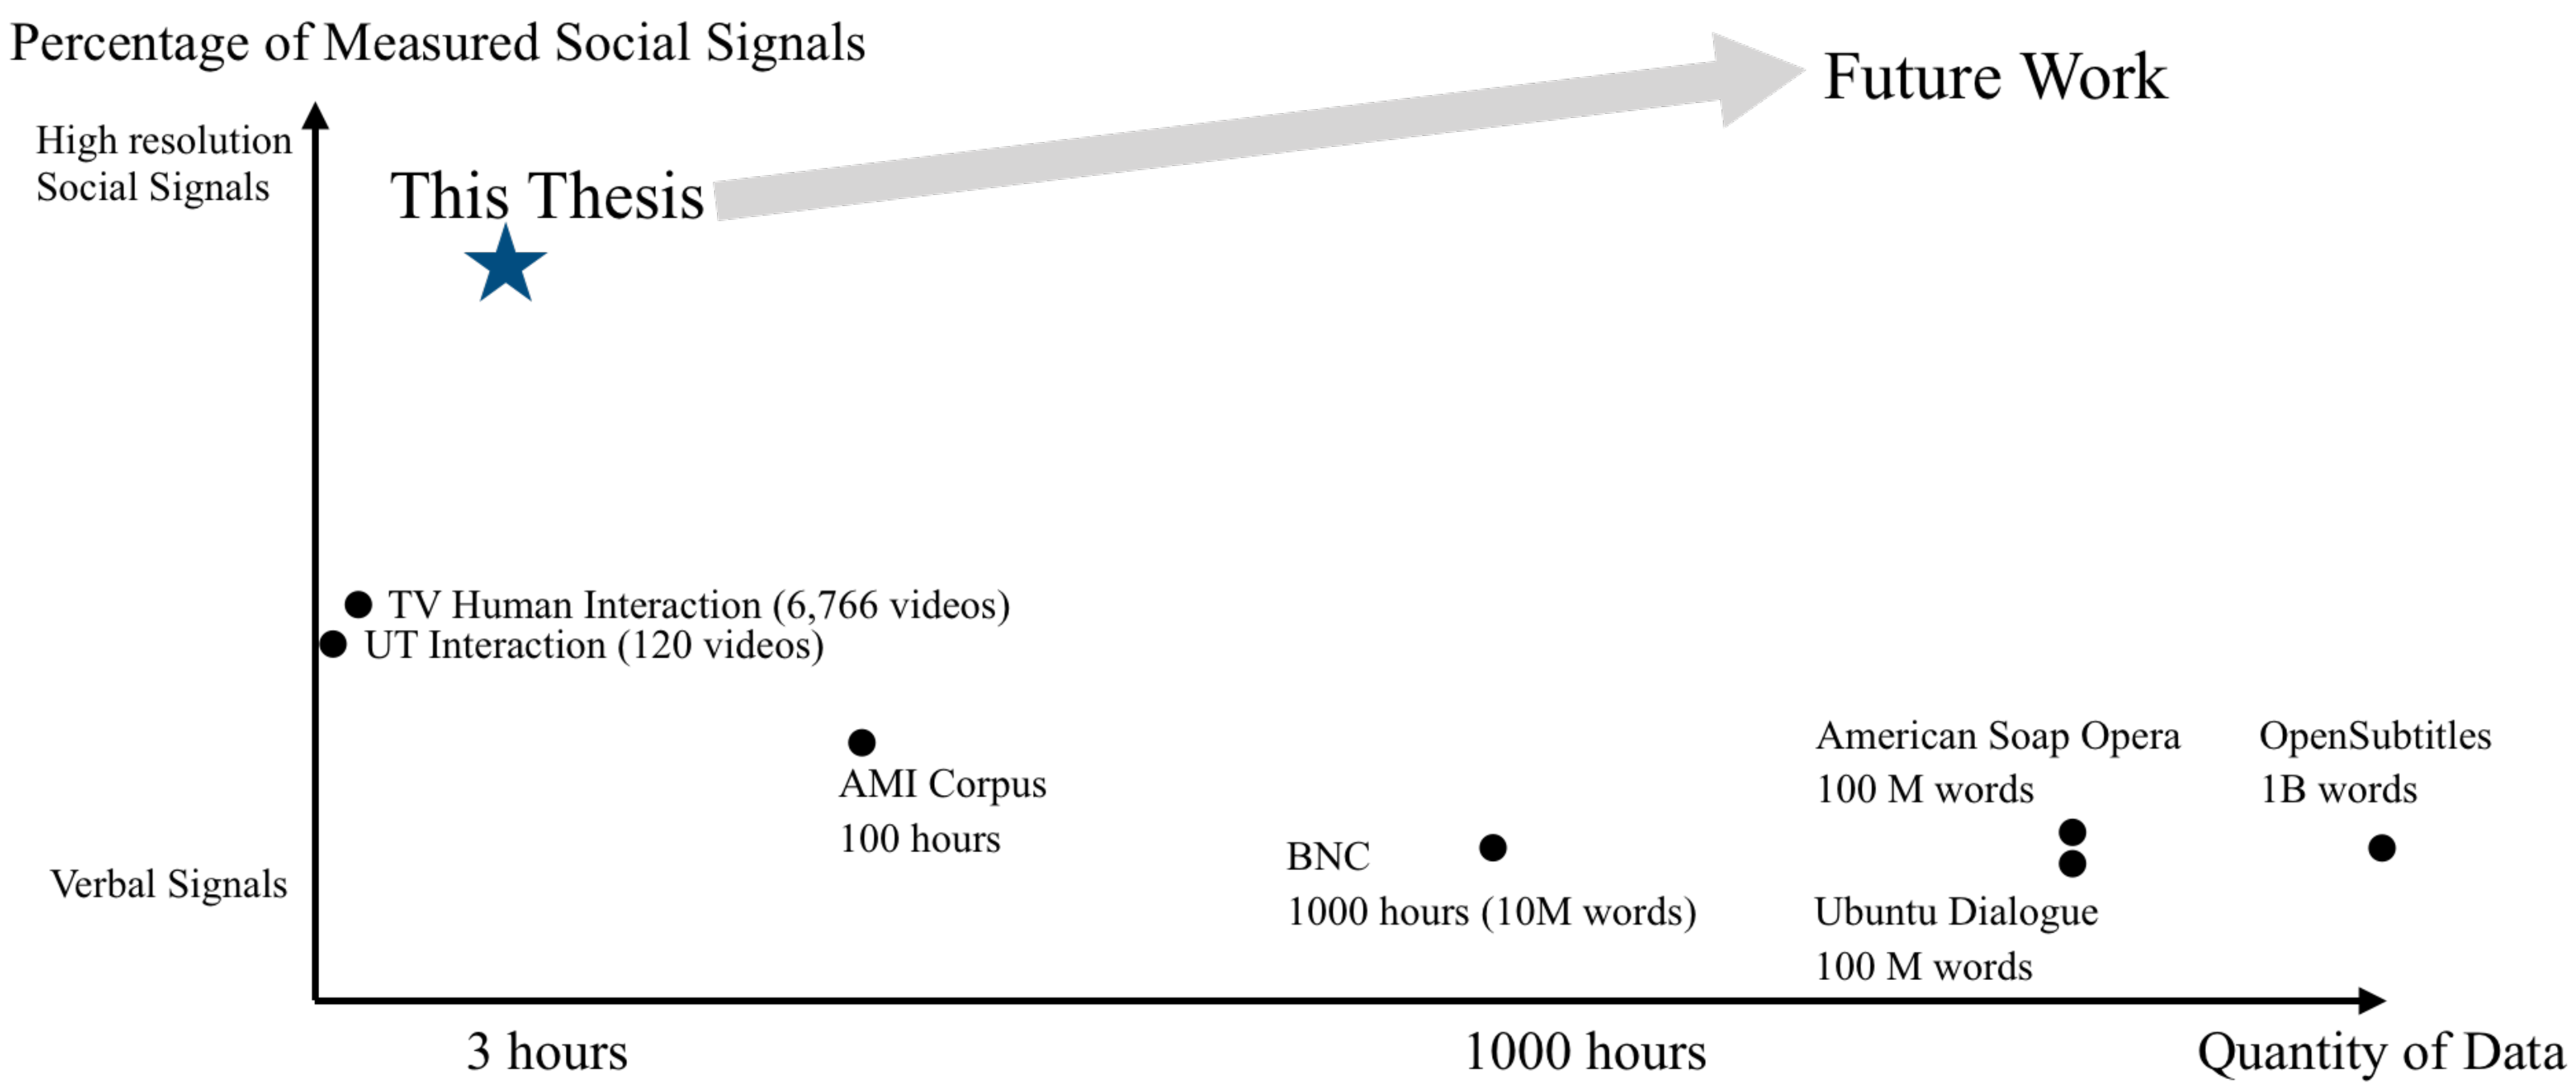
\includegraphics[width=\textwidth]{figures/summary}
	\caption{As an important contribution, this thesis enables to measure much higher dimensional social signals exchanged in genuine social interaction compared to the existing work. Collecting higher fidelity and more quantity of data is interesting future directions.}
	\label{fig:summary}
\end{figure*}

\section{Future Work}
This thesis takes the first step toward the ambitious goal of building ``social Artificial Intelligence''. As an important contribution, this thesis enables to measure much higher dimensional social signals exchanged in genuine social interaction compared to the existing work (as illustrated in Figure
~\ref{fig:summary}), and demonstrates how to use the data to computationally model nonverbal communication. We believe that there will be immense opportunities in future direction by extending the direction this thesis presents. Three key future directions are summarized below.

\paragraph{Measuring Higher Fidelity Social Signals.}
Although this thesis presents the state-of-the-art sensing and reconstruction techniques to measure social signals, the quality of the output is still not close to the level of human perception. For example, eye gaze, which plays an important role in social communication~\cite{rayner1998eye,friesen1998eyes,ricciardelli2002my}, and subtle details in the facial expressions, hairs, and clothing are missing. These are mainly caused by limited camera resolution of the system where the cameras are focusing the large working volumes. In particular, the cameras were chosen several years ago and already outdated. Although it is known that high-resolution images are extremely beneficial to reconstruct high-fidelity social signals~\cite{beeler2010high,Beeler2011}, using many high-resolution (e.g., 4K) and high-speed cameras to cover the large working volume directly introduces additional difficulties in handling and processing the larger data size. Current hand reconstruction is also vulnerable if both hands are overlapped each other, since the hand detector assumes that only a single hand is visible in a predicted bounding box. Tackling these issues is interesting future directions with many application domains, including robotics, HCI, virtual reality, and medical applications.

\paragraph{Measuring 3D Social Signals In-the-Wild.}
The Internet is a golden trove of social communication data, and these data should be utilized to model more general nonverbal communications. However, obtaining 3D signals from these in-the-wild monocular videos is a challenging problem requiring to solve the ill-posed depth ambiguity. This research may require 3D annotations for each 2D image, which cannot be reliably annotated by human annotators. We already show a promising result in this direction by presenting a monocular total capture method~\cite{Xiang2019} leveraging our Panoptic Studio database providing paired 3D skeleton annotations for images. However, this is yet only applicable to the scenes with a single person only. Capturing social signals of more complicated scenes with multiple people with better quality should be considered as a future direction to collect social signal data at scale.

\paragraph{Modeling Long-term Social Behavior in A Living Environment.}
This thesis only considers a short-term behavior by collecting database in a short social game scenario. However, interpersonal social behaviors may change over time (e.g., our behavior would be changing if we see the same person for a long time). As a future work, a long-term social behavior analysis should be also considered. This requires to capture the behaviors of the same person for a long time, and as a way, a similar multiview setup as in our Panoptic Studio needs to be installed in a living environment where humans are actually living (e.g., A camera system in a home environment). By computationally analyzing an individual's behavior in social situations for a long-term, a subject-specific model which predicts the future signals of the particular person can be trained, which can be an important property in building robots co-existing to our environment (e.g., robotic pets). As human reactions responding to the same input signals vary across people, the individual-specific prediction model can produce a distinctive output reflecting the target individual's characteristics, attending to each individual’s unique needs and goals. There are many novel scientific questions we can consider from the measurements in this new scenario including: (1) Does social familiarity influence interpersonal social behaviors; (2) How does scene affordance (e.g., furniture or TV) affect social behaviors (e.g., social formation); (3) Can long-term observations of the same person increase the social signal prediction accuracy of the particular person. 
